
\documentclass{article}

% \usepackage[spanish]{babel}

\usepackage[utf8]{inputenc}
\usepackage{graphicx}
\usepackage{amsfonts}
\usepackage{amsmath}

\title{Ecuaciones en diferencias}

\author{Alumnos de 3er semestre grupo 2}

\date{18 de septiembre de 2017}
 
\begin{document}

\maketitle

\section{Ecuaciones en diferencias}
\label{sec:ecuaciones}

% Carolina: Texto introductorio

Si en una ecuación en diferencias, la función $f$ no depende de $n$,
la ecuación en diferencias es autónoma.

\section{Ecuaciones de primer orden}

\subsection{Ecuaciones lineales}

Una ecuación lineal en diferencias de primer orden tiene la forma
$x_{n+1}=ax_n$ donde $a$ es una constante.

La fórmula para resolver ecuaciones lineales es:
\begin{equation}
  \label{lineal}
  x_n=a^nx_0.
\end{equation}

Por ejemplo, si iniciamos una inversión con 1000 pesos con un interés
mensual del 1\%, obtenemos lo siguiente:
%% Mejorar el párrafo anterior: ???????

\begin{center}
  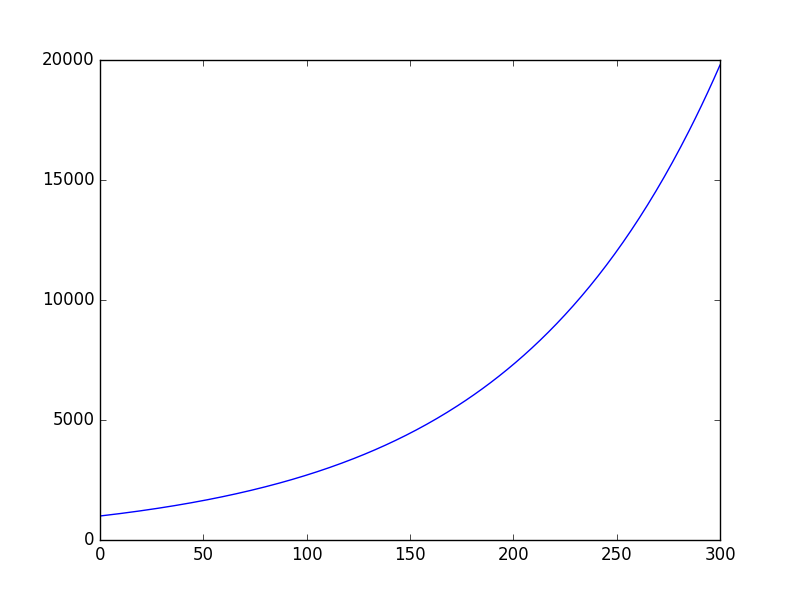
\includegraphics[width=8cm]{inversion.png}
\end{center}

Estas ecuaciones hacen que una ecuación que inicialmente era de esta
manera: $x_{n+1}=x_n+2x_n$ puede escribirse de manera que la ecuación
solo dependa de $x_n$ y queda $x_{n+1}=3x_n$, cuya solución con
condición inicial $x_0=4$ es la siguiente:
$$x_n=3^n(4).$$

\subsection{Ejemplo}

Nuestro compañerito Pepe muere en raras circunstancias (después de
tener su examen de Álgebra II), luego descubren lo radiante de su
ser. Cada 20 años el elemento radioactivo decae a razón de $2\%$, si
inicialmente contenía 165 gramos de puro amor ¿Cuánto tendrá cuando se
vea un poco más feo (como quien dice, dentro de 60 años)?

\textit{Solución:}  
Sabemos que la condición inicial es de 165 gramos y que decae un $2\%$
cada 20 años, lo cual implica que se mantiene en un $98\%$ con
respecto a al valor anterior, entonces la ecuación de diferencias de
primer orden se ve de la forma:
$$x_{n}=(.98)^n(165).$$

Ahora solo sustituimos la n por el numero deseado, en este caso
buscamos el valor del elemento cuando han pasado 60 años,
equivalentemente a $n=3$, quedando finalmente:
$$x_{3}=(.98)^3(165)= 155.29.$$

\subsection{Un ejemplito más}

% Antonio

\section{Ecuaciones de segundo orden}

Una ecuación en diferencias de segundo orden tiene la forma $a_{k+2}=f(a_k,a_{k+1})$.
El método para resolver estas ecuaciones está inspirado en la fórmula \ref{lineal}.

Para resolver una ecuación en diferencias de segundo orden se usa la ecuación resolvente.
% Mauricio



\subsection{Dos soluciones distintas}
\label{sec:distintas}
La forma en la que resolvemos una ecuación de segundo orden cuya
ecuación resolvente tenga dos raíces distintas es mediante la
siguiente formula:
\begin{equation}
 \label{raicesdistintas}
 a_n=\lambda_1x_1^n +\lambda_2x_2^n,
\end{equation}
donde $x_1$ y $x_2$ son soluciones de la ecuación de segundo orden y
$\lambda_1$ y $\lambda_2$ son escalares reales.
\subsubsection{Ejemplo}

La ecuación de segundo grado más conocida es la \textit{sucesión de
  Fibonacci}, la cual se ve de la forma:
$$a_{k+2}=a_{k+1}+a_{k},$$
en donde usualmente se toman como condiciones iniciales a: $a_{0}=1$ y $a_{1}=1$

Es inmediato calcular los primeros términos, pero ¿cómo calcularlos
cuando los términos son demasiado grandes?  Para obtenerlos,
consideramos la ecuación resolvente que viene de la ecuación original,
la cual se ve de la siguiente manera:
$$r^2-r-1=0$$

Obtenemos después ambas raíces, las cuales son:
$r_{1}= \frac{1+\sqrt{5}}{2}$ y $r_{2}=\frac{1-\sqrt{5}}{2}$. La
solución general es entonces:
$a_{k}=\alpha_{1}(\frac{1+\sqrt{5}}{2})^{k} +
\alpha_{2}(\frac{1-\sqrt{5}}{2})^k$

Ahora resolvemos un sistema de ecuaciones tal que:
$\alpha_{1} + \alpha_{2}= 1$ y
$\alpha_{1}(\frac{1+\sqrt{5}}{2}) + \alpha_{2}(\frac{1+\sqrt{5}}{2})=1$

Para obtener finalmente:
$F_{n}= \frac{5+\sqrt{5}}{10}\frac{(1+\sqrt{5})^n}{2} +
\frac{5-\sqrt{5}}{10}\frac{(1-\sqrt{5})^n}{2}$

\subsubsection{Ejemplo}
\label{sec:fichas}

¿De cuantas maneras se puede cubrir un tablero de $2\times n$ usando
fichas de $1\times 2$, $2\times 1$?

%% Explicar la solución: ???????


\subsection{Una única solución}
\label{sec:unica}

Para resolver una ecuación en diferencias de segundo orden cuya
ecuación resolvente tenga dos raíces iguales usamos la siguiente fórmula:
\begin{equation}
 \label{raicesiguales}
 a_n=\lambda_1x_1^n +\lambda_2nx_2^n,
\end{equation}
donde $x_1=x_2$ son soluciones de la ecuación de segundo orden y
$\lambda_1$ y $\lambda_2$ son escalares reales.

\subsubsection{Ejemplo}

En la siguiente ecuación en diferencias
\begin{equation}
  \label{eq:1}
  x_{n+2}=4x_{n+1}-4x_{n}
\end{equation}
veremos que la ecuación resolvente $r^2-4r+4=0$ tiene una sola raíz, a
saber: $r=2$.

La solución general es entonces:
$$x_n=\lambda_12^n+\lambda_2n2^n$$
y a continuación se deben considerar los valores iniciales para que
nos dé los valores de $\lambda_1$ y $\lambda_2$.

\subsubsection{Ejemplo}

Se plantea la siguiente ecuación en diferencias:
$a_{n+2}=2a_{n+1}-a_{n}$ con condiciones iniciales: $a_{0}=4, a_{1}=7$.

Para su solución, primero igualamos la ecuación en diferencias a
cero: $a_{n+2}-2a_{n+1}+a_{n}=0$.

Esto último nos genera una ecuación resolvente que se factoriza y
resuelve: $r^2-2r+1=0$, ${(r-1)^2=0}$, ${r=1}$.

La solución general a esta ecuación en diferencias sería:
$a_{n}=\lambda_{1}1^n+n\lambda_{2}1^n$.

Sin embargo, el problema nos da condiciones iniciales
específicas. Entonces procedemos a plantear un sistema de ecuaciones
para poder satisfacer las condiciones iniciales.
\begin{align*}
  \label{sistema2}
  a_{0}&=4=\lambda_{1}(1)^0+0\lambda_{2}(1)^0\\
  a_{1}&=7=\lambda_{1}(1)^1+1\lambda_{2}(1)^1
\end{align*}

Al resolver lo anterior obtenemos los siguientes valores:
$\lambda_{1}=4$ y $\lambda_{2}=3$, con lo que la solución final será:
$a_{n}=4(1)^n+3n(1)^n=4+3n$.


\subsection{Los números  complejos}

Un complejo es un número de la forma $z=a+bi$, $a,b\in\mathbb{R}$ ,
con $i^2=-1$, y donde $a$ recibe el nombre de parte real y $b$ el de
parte imaginaria.

El módulo de un número complejo se define como: $|a+bi|=\sqrt{a^2+b^2}$.

El argumento de un número complejo es el ángulo comprendido en(continuará)
%%% ????


\subsection{Soluciones complejas}
\label{sec:complejas}

Algunas ocasiones las ecuaciones de segundo orden no tendrán solución
en los reales, sin embargo en los complejos sí y no por manejar
números complejos su nivel de dificultad será mayor. Aquí mostramos un
ejemplo de soluciones complejas: $x_{n+2}=-4x_{n}$ con $x_0=1$ y
$x_1=0$

Resolvemos igual que en ecuaciones de segundo orden entonces aplicamos
la formula general para buscar sus raíces y tenemos: $r=\pm2i$.
Ahora buscaremos su módulo: $|r|=\sqrt{2^2}$

%%% ??????????
 
Otro ejemplo: $x_{n+2}=4x_{n+1}-8x_n$ con condiciones iniciales
$x_0=1$ y $x_1=0$. Para encontrar sus raíces se lleva a cabo el
procedimiento habitual. En este caso sus raíces son: $r=2\pm2i$

El siguiente paso es encontrar su módulo: $|r|=\sqrt{2^2+2^2}$

%%%% ???????????

\subsubsection{Ejemplo}

Para cada $n$, considera $D_{n}$ el determinante $n\times n$ dado por:

\begin{equation*}
\begin{pmatrix}
0 & 1 & 0 & 0 &\ldots & 0 & 0 & 0 & 0\\
1 & 0 & 1 & 0 &\ldots & 0 & 0 & 0 & 0\\
0 & 1 & 0 & 1 &\ldots & 0 & 0 & 0 & 0\\
0 & 0 & 1 & 0 &\ldots & 0 & 0 & 0 & 0\\
\ldots\\
0 & 0 & 0 & 0 &\ldots & 0 & 1 & 0 & 0\\
0 & 0 & 0 & 0 &\ldots & 1 & 0 & 1 & 0\\
0 & 0 & 0 & 0 &\ldots & 0 & 1 & 0 & 1\\
0 & 0 & 0 & 0 &\ldots & 0 & 0 & 1 & 0
\end{pmatrix}
\end{equation*}

%%% Solución ?????????

\subsection{Ecuaciones de segundo orden no homogéneas}
\label{sec:nohomogeneas}

%%% Teoría ???????

\subsubsection{El término no homogéneo es exponencial}
\label{sec:exponencial}

Cuando el t\'ermino no homog\'eneo es exponencial debemos proponer una soluci\'on de dicho sistema. Por ejemplo: la ecuacion en diferencias $x_{n+2}+3x_{n+1}+2x_n=3^n$ al resolver el sistema homog\'eneo obtenemos la solucion: $x-n=\lambda_1(-2)^n+\lambda_2(-1)^n$, ahora, para el sistema no homog\'eneo, debemos proponer una soluci\'on la cual es un m\'ultiplo del termino exponencial, en este ejemplo la soluci\'on del sisstema no homog\'eneo es de la forma $A(3)^n$, ya que tenemos una propuesta, debemos resolver el sistema con $x_n=A(3)^n$, veamos la soluci\'on:

\begin{align*}
  \label{solucion 32}
  A(3)^{n+2}+3A(3)^{n+1}+2A(3)^n&=(3)^n\\
  A(3)^2+3A(3)+2A&=1\\
  9A+9A+2A&=1\\
  20A&=1
\end{align*}
De ahí, concluimos que $A=\frac{1}{20}$
continuara...

\subsubsection{El término no homogéneo es polinomial}
\label{sec:polinomial}

%%% ???????????

\end{document}
